\title{Importing IGES (Initial Graphics Exchange Specification) files in ICE using Xtext}

\author{Kasper L. Gammeltoft}

\maketitle

\chapter{Introduction}


With the refactor of the Geometry Editor and Model in EAVP, it makes sense to start supporting external geometry formats in ICE. STL (Steriolithography) was simple and easy to import using a basic EMF-Based Xtext project. However, not all the geometry file formats are as easy. The IGES file format- specified in full at https://filemonger.com/specs/igs/devdept.com/version6.pdf, has its own challenges when it comes to writing an Xtext grammar to process the file. This comes in part because there are several tokens needed to parse the file that are specified in the file itself. For example the strings are specified in Hollerith Format- the string is represented as itself prefixed with the number of characters in it and an 'H'. For instance, in order to specify the strings 'Hello' or '2fn 3390', the literals are given with '5HHello' and '8H2fn 3390', respectively. It is impossible to specify an explicit grammar rule for these strings as the token changes length depending on the number at the front. Another challenge in writing a grammar for the IGES file format is the specification of the current section- it comes at the end of the line (in column 73). How could the parser distinguish which line it was reading before reading to that point? First, a detailed and effective grammar had to be written, and then a custom lexer needed to override the generated internal one to handle the variable Hollerith string format.


\chapter{Process}

\section{The Grammar}

First, I generated a new Xtext project which is found under \text{File->New->Project}... and selected Xtext Project under Xtext. I did not make the project an eclipse plug-in or buildable, as that adds unnecissary peices that are only used for builds. The grammar was written in the IGES.xtext grammar file, which generates the other necessary code for the parser. To start, there are five sections that make up the IGES file format- Start, Global, Data Entry, Parameter Data, and Terminal sections. Therefore, the grammar is split into five main rules named for each section, under the into rule simply named IGES.
\newpage
\begin{Verbatim}
grammar org.eclipse.xtext.IGES

import ``http://www.eclipse.org/emf/2002/Ecore'' as ecore
generate iGES ``http://www.eclipse.org/xtext/IGES''

IGES:
    start = Start
    global = Global
    data = Data
    parameters = Parameters
    end = End;
\end{Verbatim}

Xtext will read the grammar top to bottom, making sure there is one Start, Global, Data,Parameters, and End for the file. \\

The start section is not too tricky- just read the line and ignore it- but make sure it ends with 'S      #' and a newline, which signifies that it is a start section line.

\begin{Verbatim}
Start:
    (lines+=startLine)+;

startLine returns ecore::EString:
    (STRING | WS)* 'S' WS? INT ENDLINE;
\end{Verbatim}

The startLine rule returns a String, and uses terminal rules defined in the grammar- rules the lexer uses to break up the file before the parser reads it. The terminal rules used with the lexer are very important to the grammar:

\begin{Verbatim}
terminal INT returns ecore::EInt:
    ('0'..'9')+;

terminal DOUBLE returns ecore::EDouble:
    ('+' | '-')? INT '.' INT? (('e' | 'E') ('+' | '-')? INT)?;

	// Is implemented in CustomIGESLexer properly',' this is just declarative
terminal HOLLERITH:
    INT 'H' .;

terminal STRING:
    ('A..Z' | 'a'..'z' | '0'..'9' | '"')+;

terminal WS:
    (' ' | '\t' | '\r')+;

terminal ENDLINE:
    '\r'? '\n';
	
terminal DELIMITER:
    . ;

terminal SEPARATOR:
    . ;
\end{Verbatim}

For now, don't worry about the strange DELIMITER or SEPARATOR terminals. Those come into play with the custom lexer. So the start line now means- read an arbitrary number of terminal STRING's or WS's, then look for the pattern:
\begin{Verbatim}
'S' WS? INT ENDLINE
\end{Verbatim}

  This means there must be an S with optional whitespace followed by an integer followed by a newline. \\
  Next is the global section, which contains the Hollerith strings. For now, just trust that the terminal Hollerith will work, and the following grammar will be able to parse the IGES file:

\begin{Verbatim}
Global:
    {Global}
    DELIMITER? HString? DELIMITER?
    ((values+=Value)*  WS? 'G' WS? INT ENDLINE)+
    (values+=Value)* SEPARATOR WS? 'G' WS? INT ENDLINE;
\end{Verbatim}

The global section contains parameters for the file in a delimiter-separated list, which can span multiple lines. The list is over when indicated by a specified separator.

The \begin{Verbatim}
DELIMITER? HString? DELIMITER?
\end{Verbatim}

indicates the ambiguity of IGES files. The first value in the list of parameters for the global section is the delimiter itself. For example, given the global section:

\begin{Verbatim}
1H,,1H;,4HSLOT, ...     G       1
\end{Verbatim}

The delimiter is specified as the comma (1H,), and the separator as the semicolon (1H;). But, if these values are omitted, the default comma and semicolon are assumed. Therefore, there are several options for specifying the same information:\\
1H,,1H;,4HSLOT\\
1H,,,4HSLOT\\
,1H;,4HSLOT\\
,,4HSLOT\\
All four indicate the default delimiter and separator value of the comma and semicolon, respectively. The 4HSLOT, being the third value in the list, indicates the name of the geometry. \\
Finally, there are an arbitrary number of values followed by the end of the line- similar to the start lines. Finally, the last global line is indicated by the separator after the last value in the list.\\
After that, the data is read in through the two middle sections. The data entry section has a precise specification- each entity has 20 fields and each field means the same thing for any entity. Therefore, reading in these was easy:
\begin{Verbatim}
Data:
    (entries+=Entry)+;

Entry:
    WS type=INT WS? paramData=INT WS? structure=INT WS? lineFont=INT WS? level=INT WS?
    view=INT WS? TransformMatrix=INT WS? INT? WS? status=INT 'D' WS? index=INT ENDLINE
    WS? INT WS? lineWeight=INT WS? color=INT WS? paramLines=INT WS? form=INT WS?
    (entityLabel=STRING)? WS? subNum=INT 'D' WS? INT ENDLINE;
\end{Verbatim}

  The first line of the declaration has ten fields (type, paramData, etc.) as does the second (lineweight, color, etc.). These are just read in as ints, except for the possible entity label, which can be a string.

  The parameter data section is more similar to the global data section, as it contains delimiter separated lists of values for the given entity. The list starts with the type of entity, and is on the same line given by the paramData value for each Entry above.

\begin{Verbatim}
Parameters:
    (entries+=(PMultiEntry | PEntry))+;

PEntry:
    type=INT DELIMITER?
    (values+=Value)* SEPARATOR WS? dIndex=INT 'P' WS? indicies+=INT ENDLINE;

PMultiEntry returns PEntry:
    type=INT DELIMITER?
    ((values+=Value)* WS? dIndex=INT 'P' WS? indicies+=INT ENDLINE)+
    (values+=Value)* SEPARATOR WS? INT 'P' WS? INT ENDLINE;
\end{Verbatim}

This allows for either single line or multi-line parameter data specifications. The last line is specified by having the SEPARATOR after its last value. The Value rule was also used for the Global data section's data, and is declared as delimiter separated values that are either Hollerith Strings, double-precision floating point numbers, or integers. They are defined like this:
\begin{Verbatim}
Value:
    Param | Pointer | HString;

HString:
    val=HOLLERITH DELIMITER?;

Param:
    val=DOUBLE DELIMITER?;

Pointer:
    val=INT DELIMITER?;
\end{Verbatim}

Finally, the End section is just a single line with the total line numbers of the other sections. It can be easily specified with this:
\begin{Verbatim}
End:
    'S' WS? sval=INT 'G' WS? gval=INT 'D' WS? dval=INT
    'P' WS? pval=INT WS 'T' WS? tval=INT;
\end{Verbatim}

The grammar is thus a set of all subgrammars- each section is broken down into fundamental rules and compiled to form the total IGES grammar. Here is the entire thing:

\begin{Verbatim}
grammar org.eclipse.xtext.IGES

import "http://www.eclipse.org/emf/2002/Ecore" as ecore
generate iGES "http://www.eclipse.org/xtext/IGES"

IGES:
    start=Start
    global=Global
    data=Data
    parameters=Parameters
    end=End;

Start:
    (lines+=startLine)+;

Global:
    {Global}
    DELIMITER? HString? DELIMITER?
    ((values+=Value)*  WS? 'G' WS? INT ENDLINE)+
    (values+=Value)* SEPARATOR WS? 'G' WS? INT ENDLINE;

Data:
    (entries+=Entry)+;

Entry:
    WS type=INT WS? paramData=INT WS? structure=INT WS? lineFont=INT WS? level=INT WS?
    view=INT WS? TransformMatrix=INT WS? INT? WS? status=INT 'D' WS? index=INT ENDLINE
    WS? INT WS? lineWeight=INT WS? color=INT WS? paramLines=INT WS? form=INT WS?
    (entityLabel=STRING)? WS? subNum=INT 'D' WS? INT ENDLINE;

Parameters:
    (entries+=(PMultiEntry | PEntry))+;

PEntry:
    type=INT DELIMITER?
    (values+=Value)* SEPARATOR WS? dIndex=INT 'P' WS? indicies+=INT ENDLINE;

PMultiEntry returns PEntry:
    type=INT DELIMITER?
    ((values+=Value)* WS? dIndex=INT 'P' WS? indicies+=INT ENDLINE)+
    (values+=Value)* SEPARATOR WS? INT 'P' WS? INT ENDLINE;

Value:
    Param | Pointer | HString;

HString:
    val=HOLLERITH DELIMITER?;

Param:
    val=DOUBLE DELIMITER?;

Pointer:
    val=INT DELIMITER?;

End:
    'S' WS? sval=INT 'G' WS? gval=INT 'D' WS? dval=INT
    'P' WS? pval=INT WS 'T' WS? tval=INT;

startLine returns ecore::EString:
    (STRING | WS)* 'S' WS? INT ENDLINE;

terminal INT returns ecore::EInt:
    ('0'..'9')+;

terminal DOUBLE returns ecore::EDouble:
    ('+' | '-')? INT '.' INT? (('e' | 'E') ('+' | '-')? INT)?;

terminal HOLLERITH:
    INT 'H' .;

terminal STRING:
    ('A..Z' | 'a'..'z' | '0'..'9' | '"')+;

terminal WS:
    (' ' | '\t' | '\r')+;

terminal ENDLINE:
    '\r'? '\n';
	
terminal DELIMITER:
    . ;

terminal SEPARATOR:
    . ;
\end{Verbatim}

\section{Extending the Generated Lexer}

Xtext creates a lexer from the grammar given to parse the file. However, the default lexer does not have the ability to handle variable length strings or non-literal delimiter strings. Therefore a custom lexer needs to handle the Hollerith and delimiter strings, rather than the generated internal lexer. To do this, we can extend the old lexer, add the changes we need, and bind our new lexer to Xtext as the runtime lexer.\\

First, I created a new lexer that extended the current InternalIGESLexer.java (which should be located in org.eclipse.xtext.parser.antlr.internal in the src-gen folder). I named the new lexer CustomIGESLexer.java, and placed it in the src/org.eclipse.xtext package. The first thing to do is to override the mTokens() function, which decides which lexer rule to call given the current stream input. We want to call our own functions for the hollerith, delimiter, and separator rules:

\begin{Verbatim}
    @Override 
    public void mTokens() throws RecognitionException{
        // If the token is hollerith, read it as hollerith
    	if (isHollerith()){
            // If delimieter is not set, this must be it
    	    if (DELIMITER == null) {
    	        setDelimiter();
                // Flag helping set separator properly
    		DELIM_SET = true;
            // If the separator is not set, then this must be it
    	    } else if (SEPARATOR == null) {
    		setSEPARATOR();
    	    }
        // Do the rule for hollerith strings
    	RULE_HOLLERITH();
        // Do the rule for the delimiter
    	} else if (isDelimiter()) {
    		
	    RULE_DELIMITER();
        // Do the rule for the separator
    	} else if (isSEPARATOR()) {
    		
	    RULE_SEPARATOR();
        // Delegate to the internal lexer for all other tokens
        } else {
    	    super.mTokens();
    	}
    }
\end{Verbatim}

Setting aside the delimiter and separator, the Hollerith rule is simple enough to implement. We want to read the integer in the front, then an 'H' character, then read the next n (where n = int at front) characters. Here is the definition of the HOLLERITH terminal rule:


\begin{Verbatim}
public final void RULE_HOLLERITH() throws RecognitionException {
    try {
        // Follow style and conventions of internal lexer
	int _type = RULE_HOLLERITH;
	int _channel = DEFAULT_TOKEN_CHANNEL;

	// Read in the int at the beginning of the string
	String curInt = "";
	// Get the next character
	int cur = input.LA(1);
	// While it is a digit add it to cur
	while (cur >= '0' && cur <= '9') {
	    curInt += (char) cur;
	    matchRange('0', '9');
	    cur = input.LA(1);
	}
	// Try to read the integer. Should be successful. Otherwise there
	// was an error
	int n;
	try {
	    n = Integer.parseInt(curInt);
	} catch (Exception e) {
	    throw new EarlyExitException(1, input);
        }

	// Match the H
	match('H');

	// Match the n number of characters in the stream
	for (int i = 0; i < n; i++) {
	    matchAny();
	}
        // Set the type and channel, as the internal lexer does
	state.type = _type;
	state.channel = _channel;
    } finally {
    }
}
\end{Verbatim}

Checking if a string is a hollerith or not simply checks for an integer followed by 'H':

\begin{Verbatim}
    private boolean isHollerith() {
	int index = 1;
	int cur = input.LA(index);

	while (cur >= '0' && cur <= '9') {
            index++;
	    cur = input.LA(index);
	}
	return index > 1 && cur == 'H';
    }
\end{Verbatim}

Now the hollerith strings will be handled by our lexer, once it is bound to the xtext project. To do this, we open up the IGESRuntimeModule.java or IGESRuntimeModule.xtend and add the following code:\\
Java:
\begin{Verbatim}
    @Override
    public void configureRuntimeLexer(Binder binder) {
	binder.bind(Lexer.class)
	    .annotatedWith(Names.named(LexerBindings.RUNTIME))
	    .to(CustomIGESLexer.class);
    }
\end{Verbatim}

Xtend:

\begin{Verbatim}
    override public void configureRuntimeLexer(Binder binder) {
	binder.bind(Lexer)
	    .annotatedWith(Names.named(LexerBindings.RUNTIME))
	    .to(CustomIGESLexer);
    }
\end{Verbatim}

Now the runtime lexer for the IGES files will be the custom IGES lexer! Only one thing left to figure out- getting custom delimiters to work.\\
The custom delimiters is a challenging problem, but with some assumptions we can handle it. The first assumption is that the delimiter will be reasonable- as in not letters or numbers which are mistaken for strings and, well, numbers. The second assumption is that the start lines, above the global section, do not contain any tricky tokens, such as hollerith strings or commas. Now, back to the mTokens() method. We saw that the delimiter is set as the first hollerith, and the separator as the second. But if they are left blank, we still need to set them with the default values. Lets look at the three methods for delimiter (and separator): isDelimiter(), setDelimiter(), and the rule DELIMITER. Adding the instance variables to the top of the class definition:

\begin{Verbatim}
    private String DELIMITER = null;
    private String SEPARATOR = null;
    boolean DELIM_SET = false;
\end{Verbatim}

Now for the isDelimiter() method, we want to check the characters of the delimiter against the current token.

\begin{Verbatim}
    private boolean isDelimiter() {
        if (DELIMITER == null) {
	    return false;
	}
	int index = 0;

	while (index < DELIMITER.length() && (input.LA(index + 1)) == DELIMITER.charAt(index)) {
	    index++;
	}
	return index == DELIMITER.length();
    }
\end{Verbatim}

The setDelimiter() method simply gets the hollerith string and sets the instance variable:

\begin{Verbatim}
    private void setDelimiter() {
	String curInt = "";
	int index = 1;
	int cur = input.LA(index);
	while (cur >= '0' && cur <= '9') {
	    curInt += (char) cur;
	    index++;
	    cur = input.LA(index);
	}
	int n;
	try {
	    n = Integer.parseInt(curInt);
	} catch (Exception e) {
	    e.printStackTrace();
	    return;
	}

	if (input.LA(index) == 'H') {
	    index++;
	} else {
	    return;
	}
	DELIMITER = "";
	for (int i = 0; i < n; i++) {
	    DELIMITER += (char) input.LA(index + i);
	}
    }
\end{Verbatim}

And finally, the rule DELIMITER just matches the characters for the lexer:

\begin{Verbatim}
    public final void RULE_DELIMITER() throws RecognitionException {
	try {
	    int _type = RULE_DELIMITER;
	    int _channel = DEFAULT_TOKEN_CHANNEL;

	    for (int i = 0; i < DELIMITER.length(); i++) {
		match(String.valueOf(DELIMITER.charAt(i)));
            }

	    if (SEPARATOR == null && !DELIM_SET) {
                SEPARATOR = ";";
	    }

            DELIM_SET = false;
                
            state.type = _type;
            state.channel = _channel;
	} finally {
	}
    }
\end{Verbatim}

The delimiter rule also will set the separator if it needs to be set. This would happen when the delimiter has been set, but there is no value for the separator afterward, so the rule delimiter is called immediately after. In this case, the delimiter rule should set the separator. The separator has almost identical functions to these. Now, we just need to add the case of empty values for the delimiter and separator in the mTokens() method:

\begin{Verbatim}
    @Override
    public void mTokens() throws RecognitionException {
	if (isHollerith()) {
	    if (DELIMITER == null) {
		setDelimiter();
		DELIM_SET = true;
	    } else if (SEPARATOR == null) {
		setSEPARATOR();
	}
	    RULE_HOLLERITH();

	} else if (isDelimiter()) {

	    RULE_DELIMITER();

	} else if (isSEPARATOR()) {
0
	    RULE_SEPARATOR();
	} else {
	    if (isComma() && DELIMITER == null) {
		DELIMITER = ",";
		super.mRULE_DELIMITER();
	    } else {
	        super.mTokens();
	    }
	}
    }
\end{Verbatim}

Now the lexer will be able to handle the hollerith strings as well as the variable delimiters. Here is the whole CustomIGESLexer.java:

\begin{Verbatim}
package org.eclipse.january.geometry.xtext;

import org.eclipse.january.geometry.xtext.parser.antlr.internal.InternalIGESLexer;

import org.antlr.runtime.*;


/**
 * This class provides custom functions for properly lexing IGES files. The Hollerith,
 * Delimiter, and Separator terminal functions are implemented here, but there definitions
 * in the grammar are important to match for the parser. 
 * @author Kasper Gammeltoft
 *
 */
public class CustomIGESLexer extends InternalIGESLexer {

	/** The delimiter for the lexer */
	private String DELIMITER = null;
	/** The entry separator for the lexer */
	private String SEPARATOR = null;
	/**
	 * Flag indicating if the delimiter was specified in the file. This
	 * determines if the separator needs to be set to default ';' when the
	 * delimiter is called again.
	 */
	boolean DELIM_SET = false;

	public CustomIGESLexer() {
		;
	}

	public CustomIGESLexer(CharStream input) {
		this(input, new RecognizerSharedState());
	}

	public CustomIGESLexer(CharStream input, RecognizerSharedState state) {
		super(input, state);

	}

	@Override
	/*
	 * (non-Javadoc)
	 * 
	 * @see org.eclipse.january.geometry.xtext.parser.antlr.internal.
	 * InternalIGESLexer#mTokens()
	 */
	public void mTokens() throws RecognitionException {
		// Handle hollerith string
		if (isHollerith()) {
			
			// Delimiter needs to be set first
			if (DELIMITER == null) {
				setDelimiter();
				
				// Set flag to true
				DELIM_SET = true;
				
			// Separator is second
			} else if (SEPARATOR == null) {
				setSEPARATOR();
			}
			// Call the new Hollerith rule
			RULE_HOLLERITH();
			
		// process the delimiter
		} else if (isDelimiter()) {
			RULE_DELIMITER();
			
		// process the separator
		} else if (isSEPARATOR()) {
			RULE_SEPARATOR();
		// Other token
		} else {
			// If comma, then check delimiter
			if (isComma() && DELIMITER == null) {
				// Set the delimiter as default
				DELIMITER = ",";
				super.mRULE_DELIMITER();
				// Let all other tokens be handled
				// by internal lexer
			} else {
				super.mTokens();
			}
		}
	}

	/**
	 * Determines if the current token on the stream is the delimiter for the
	 * current file
	 * 
	 * @return Returns true if the token is the delimiter, false if otherwise
	 */
	private boolean isDelimiter() {
		// Cannot be if delimiter is null
		if (DELIMITER == null) {
			return false;
		}
		
		int index = 0;
		// Check each character
		while (index < DELIMITER.length() && (input.LA(index + 1)) == DELIMITER.charAt(index)) {
			index++;
		}
		// Return if index got to end or not
		return index == DELIMITER.length();
	}

	/**
	 * Determines if the current token on the stream is the separator for the
	 * current file
	 * 
	 * @return Returns true if the token is the separator, false if otherwise
	 */
	private boolean isSEPARATOR() {
		// Cannot be if separator is null
		if (SEPARATOR == null) {
			return false;
		}
		int index = 0;
		// Check each character
		while (index < SEPARATOR.length() && (input.LA(index + 1)) == SEPARATOR.charAt(index)) {
			index++;
		}
		// Return if index got to the end or not
		return index == SEPARATOR.length();
	}

	/**
	 * Sets the delimiter for the current file.
	 */
	private void setDelimiter() {
		// Setup temp string
		String curInt = "";
		int index = 1;
		int cur = input.LA(index);
		// get hollerith string length
		while (cur >= '0' && cur <= '9') {
			curInt += (char) cur;
			index++;
			cur = input.LA(index);
		}
		// Get int value
		int n;
		try {
			n = Integer.parseInt(curInt);
		} catch (Exception e) {
			e.printStackTrace();
			return;
		}
		// Make sure it is a hollerith
		if (input.LA(index) == 'H') {
			index++;
		} else {
			return;
		}
		// Set the delimiter
		DELIMITER = "";
		for (int i = 0; i < n; i++) {
			DELIMITER += (char) input.LA(index + i);
		}
	}

	/**
	 * Sets the separator for the current file.
	 */
	private void setSEPARATOR() {
		// Setup temp string
		String curInt = "";
		int index = 1;
		int cur = input.LA(index);
		// Get hollerith string length
		while (cur >= '0' && cur <= '9') {
			curInt += (char) cur;
			index++;
			cur = input.LA(index);
		}
		// Get int value
		int n;
		try {
			n = Integer.parseInt(curInt);
		} catch (Exception e) {
			e.printStackTrace();
			return;
		}
		
		// Make sure it is a hollerith string
		if (input.LA(index) == 'H') {
			index++;
		} else {
			return;
		}
		// Set the separator
		SEPARATOR = "";
		for (int i = 0; i < n; i++) {
			SEPARATOR += (char) input.LA(index + i);
		}

	}

	/**
	 * Custom lexer rule for the delimiter token. Matches the file specified
	 * entry delimiter.
	 * 
	 * @throws RecognitionException
	 */
	public final void RULE_DELIMITER() throws RecognitionException {
		try {
			int _type = RULE_DELIMITER;
			int _channel = DEFAULT_TOKEN_CHANNEL;

			{	
				// Match the delimiter in the token stream
				for (int i = 0; i < DELIMITER.length(); i++) {
					match(String.valueOf(DELIMITER.charAt(i)));
				}
				// If the separator is not set, and needs to be, then set it
				if (SEPARATOR == null && !DELIM_SET) {
					SEPARATOR = ";";
				}

                                // Delimiter has already been set
                                DELIM_SET = false;

			}

			state.type = _type;
			state.channel = _channel;
		} finally {
		}
	}

	/**
	 * Custom lexer rule for the separator token. Matches the file specified
	 * entry separator.
	 * 
	 * @throws RecognitionException
	 */
	public final void RULE_SEPARATOR() throws RecognitionException {
		try {
			int _type = RULE_SEPARATOR;
			int _channel = DEFAULT_TOKEN_CHANNEL;

			{
				// Match the separator in the token stream
				for (int i = 0; i < SEPARATOR.length(); i++) {
					match(String.valueOf(SEPARATOR.charAt(i)));
				}

			}

			state.type = _type;
			state.channel = _channel;
		} finally {
		}
	}

	/**
	 * Custom lexer rule for getting Hollerith strings. Is not dictated by the
	 * grammar! Will return the entire Hollerith string, including the int 'H'
	 * prefix.
	 * 
	 * @throws RecognitionException
	 */
	public final void RULE_HOLLERITH() throws RecognitionException {
		try {
			// Follow style and conventions of internal lexer
			int _type = RULE_HOLLERITH;
			int _channel = DEFAULT_TOKEN_CHANNEL;

			// Read in the int at the beginning of the string
			String curInt = "";
			// Get the next character
			int cur = input.LA(1);
			// While it is a digit add it to cur
			while (cur >= '0' && cur <= '9') {
				curInt += (char) cur;
				matchRange('0', '9');
				cur = input.LA(1);
			}
			// Try to read the integer. Should be successful. Otherwise there
			// was an error
			int n;
			try {
				n = Integer.parseInt(curInt);
			} catch (Exception e) {
				throw new EarlyExitException(1, input);
			}

			// Match the H
			match('H');

			// Match the n number of characters in the stream
			for (int i = 0; i < n; i++) {
				matchAny();
			}
			// Set the type and channel, as the internal lexer does
			state.type = _type;
			state.channel = _channel;
		} finally {
		}
	}

	/**
	 * Checks if the current token is a Hollerith String
	 * 
	 * @return Returns true if the current token is a Hollerith string, false if
	 *         otherwise
	 */
	private boolean isHollerith() {
		int index = 1;
		int cur = input.LA(index);
		// See if an int starts the string
		while (cur >= '0' && cur <= '9') {
			index++;
			cur = input.LA(index);
		}
		// Followed by an 'H'
		return index > 1 && cur == 'H';
	}

	/**
	 * Checks if the current character in the stream is a comma
	 * 
	 * @return Returns true if it is a comma, false if otherwise
	 */
	private boolean isComma() {

		return (input.LA(1) == ',');

	}

}
\end{Verbatim}

\chapter{Result}

The IGES format can now be understood by Xtext with the grammar and custom lexer provided. Using these tools to import an IGES file can return an IGES data populated with each of the start, global, data, parameters, and end variables, which in turn contain the document data. Xtext also offers editors for Eclipse which can comprehend the language we specified. However, there is still some work to test and properly visualize these IGES files.

\section{Testing}

Xtext automatically creates a testing bundle when making a new XText project. Under the ..xtext.iges.tests bundle, add a new JUnit test in the src folder. I also added a testing file for the JUnit to test against, the example file on Wikipedia is a good start. Now to import the file using Xtext, instantiate a new standalone xtext parser and create resources from it with the example file:

\begin{Verbatim}
    Injector injector = new IGESStandaloneSetup().createInjectorAndDoEMFRegistration();
    XtextResourceSet resourceSet = injector.getInstance(XtextResourceSet.class);
    resourceSet.addLoadOption(XtextResource.OPTION_RESOLVE_ALL, Boolean.TRUE);
    Resource resource = resourceSet.getResource(URI.createFileURI(path.toFile()
       .getAbsolutePath()), true);
\end{Verbatim}

Now get the first resource from the resource set- it should be an IGES instance from the EMF model, with all the loaded data. Test the data from the resource against the file contents to see if everything imported properly. Here is the test code I wrote for the file on Wikipedia:

\newpage

\begin{Verbatim}
private void testIGES(IGES data) {
	Start s = data.getStart();
	assertEquals(1, s.getLines().size());
		
	String sl = s.getLines().get(0);
	assertEquals(
        "                                                                       " +
           "S      1\n", sl);
		
	Global g = data.getGlobal();
		
	List<Value> gv = g.getValues();
	assertEquals(23, gv.size());
	    
	assertEquals("1H;", ((HString)gv.get(0)).getVal());
	assertEquals("4HSLOT", ((HString)gv.get(1)).getVal());
	assertEquals("37H$1$DUA2:[IGESLIB.BDRAFT.B2I]SLOT.IGS;",
            ((HString)gv.get(2)).getVal());
	assertEquals("17HBravo3 BravoDRAFT", ((HString)gv.get(3)).getVal());
	assertEquals("31HBravo3->IGES V3.002 (02-Oct-87)", ((HString)gv.get(4)).getVal());
	assertEquals(32, ((Pointer)gv.get(5)).getVal());
	assertEquals(38, ((Pointer)gv.get(6)).getVal());
	assertEquals(6, ((Pointer)gv.get(7)).getVal());
	assertEquals(38, ((Pointer)gv.get(8)).getVal());
	assertEquals(15, ((Pointer)gv.get(9)).getVal());
	assertEquals("4HSLOT", ((HString)gv.get(10)).getVal());
	assertEquals(1.0, ((Param)gv.get(11)).getVal(), 0.0);
	assertEquals(1, ((Pointer)gv.get(12)).getVal());
        // ...
	// If all those are correct, check last values and move on
	
	assertEquals("24HAPPLICON - Ann Arbor, MI", ((HString)gv.get(20)).getVal());
	assertEquals(4, ((Pointer)gv.get(21)).getVal());
	assertEquals(0, ((Pointer)gv.get(22)).getVal());
	
	
	Data d = data.getData();
	
	List<Entry> de = d.getEntries();
	
	assertEquals(6, de.size());

	checkEntry(de.get(0), 116, 1, 0, 1, 0, 0, 0, 1, 1, 1, 5, 1, 0, null, 0);
	checkEntry(de.get(1), 116, 2, 0, 1, 0, 0, 0, 1, 3, 1, 5, 1, 0, null, 0);
	checkEntry(de.get(2), 100, 3, 0, 1, 0, 0, 0, 1, 5, 1, 2, 1, 0, null, 0);
	checkEntry(de.get(3), 100, 4, 0, 1, 0, 0, 0, 1, 7, 1, 2, 1, 0, null, 0);
	checkEntry(de.get(4), 110, 5, 0, 1, 0, 0, 0, 1, 9, 1, 3, 1, 0, null, 0);
	checkEntry(de.get(5), 110, 6, 0, 1, 0, 0, 0, 1, 11, 1, 3, 1, 0, null, 0);
	
	Parameters p = data.getParameters();
	
	List<PEntry> pe = p.getEntries();
	
	assertEquals(6, pe.size());
	
	PEntry p1 = pe.get(0);
	assertEquals(116, p1.getType());
	
	List<Value> p1v = p1.getValues();
	assertEquals(6, p1v.size());
	
	assertEquals(0.0, ((Param)p1v.get(0)).getVal(), 0.0);
	assertEquals(0.0, ((Param)p1v.get(1)).getVal(), 0.0);
	assertEquals(0.0, ((Param)p1v.get(2)).getVal(), 0.0);
	assertEquals(0, ((Pointer)p1v.get(3)).getVal());
	assertEquals(0, ((Pointer)p1v.get(4)).getVal());
	assertEquals(0, ((Pointer)p1v.get(5)).getVal());
	
	PEntry p2 = pe.get(1);
	assertEquals(116, p2.getType());
	
	List<Value> p2v = p2.getValues();
	assertEquals(6, p2v.size());
	
	assertEquals(5.0, ((Param)p2v.get(0)).getVal(), 0.0);
	assertEquals(0.0, ((Param)p2v.get(1)).getVal(), 0.0);
	assertEquals(0.0, ((Param)p2v.get(2)).getVal(), 0.0);
	assertEquals(0, ((Pointer)p2v.get(3)).getVal());
	assertEquals(0, ((Pointer)p2v.get(4)).getVal());
	assertEquals(0, ((Pointer)p2v.get(5)).getVal());
	
	PEntry p3 = pe.get(2);
	assertEquals(100, p3.getType());
	
	List<Value> p3v = p3.getValues();
	assertEquals(9, p3v.size());
	
	assertEquals(0.0, ((Param)p3v.get(0)).getVal(), 0.0);
	assertEquals(0.0, ((Param)p3v.get(1)).getVal(), 0.0);
	assertEquals(0.0, ((Param)p3v.get(2)).getVal(), 0.0);
	assertEquals(0.0, ((Param)p3v.get(3)).getVal(), 0.0);
	assertEquals(1.0, ((Param)p3v.get(4)).getVal(), 0.0);
	assertEquals(0.0, ((Param)p3v.get(5)).getVal(), 0.0);
	assertEquals(-1.0, ((Param)p3v.get(6)).getVal(), 0.0);
	assertEquals(0, ((Pointer)p3v.get(7)).getVal());
	assertEquals(0, ((Pointer)p3v.get(8)).getVal());
	
	PEntry p4 = pe.get(3);
	assertEquals(100, p4.getType());
	
	List<Value> p4v = p4.getValues();
	assertEquals(9, p4v.size());
	
	assertEquals(0.0, ((Param)p4v.get(0)).getVal(), 0.0);
	assertEquals(5.0, ((Param)p4v.get(1)).getVal(), 0.0);
	assertEquals(0.0, ((Param)p4v.get(2)).getVal(), 0.0);
	assertEquals(5.0, ((Param)p4v.get(3)).getVal(), 0.0);
	assertEquals(-1.0, ((Param)p4v.get(4)).getVal(), 0.0);
	assertEquals(5.0, ((Param)p4v.get(5)).getVal(), 0.0);
	assertEquals(1.0, ((Param)p4v.get(6)).getVal(), 0.0);
	assertEquals(0, ((Pointer)p4v.get(7)).getVal());
	assertEquals(0, ((Pointer)p4v.get(8)).getVal());
	
	PEntry p5 = pe.get(4);
	assertEquals(110, p5.getType());
	
	List<Value> p5v = p5.getValues();
	assertEquals(8, p5v.size());
	
	assertEquals(0.0, ((Param)p5v.get(0)).getVal(), 0.0);
	assertEquals(-1.0, ((Param)p5v.get(1)).getVal(), 0.0);
	assertEquals(0.0, ((Param)p5v.get(2)).getVal(), 0.0);
	assertEquals(5.0, ((Param)p5v.get(3)).getVal(), 0.0);
	assertEquals(-1.0, ((Param)p5v.get(4)).getVal(), 0.0);
	assertEquals(0.0, ((Param)p5v.get(5)).getVal(), 0.0);
	assertEquals(0, ((Pointer)p5v.get(6)).getVal());
	assertEquals(0, ((Pointer)p5v.get(7)).getVal());
	
	PEntry p6 = pe.get(5);
	assertEquals(110, p6.getType());
	
	List<Value> p6v = p6.getValues();
	assertEquals(8, p6v.size());
	
	assertEquals(0.0, ((Param)p6v.get(0)).getVal(), 0.0);
	assertEquals(1.0, ((Param)p6v.get(1)).getVal(), 0.0);
	assertEquals(0.0, ((Param)p6v.get(2)).getVal(), 0.0);
	assertEquals(5.0, ((Param)p6v.get(3)).getVal(), 0.0);
	assertEquals(1.0, ((Param)p6v.get(4)).getVal(), 0.0);
	assertEquals(0.0, ((Param)p6v.get(5)).getVal(), 0.0);
	assertEquals(0, ((Pointer)p6v.get(6)).getVal());
	assertEquals(0, ((Pointer)p6v.get(7)).getVal());

	End e = data.getEnd();
	
	assertEquals(1,  e.getSval());
	assertEquals(4, e.getGval());
	assertEquals(12, e.getDval());
	assertEquals(6, e.getPval());
	assertEquals(1, e.getTval());
}
	
private void checkEntry(Entry entry, int type, int param, int struct, int linefont, 
            int level, int view, int matrix, int statNum, int index, int lineweight, 
	    int color, int paramlines, int form, String label, int subNum) {
	assertEquals(type, entry.getType());
	assertEquals(param, entry.getParamData());
	assertEquals(struct, entry.getStructure());
	assertEquals(linefont, entry.getLineFont());
	assertEquals(level, entry.getLevel());
	assertEquals(view, entry.getView());
	assertEquals(matrix, entry.getTransformMatrix());
	assertEquals(statNum, entry.getStatus());
        assertEquals(index, entry.getIndex());
	assertEquals(lineweight, entry.getLineWeight());
	assertEquals(color, entry.getColor());
	assertEquals(paramlines, entry.getParamLines());
	assertEquals(form, entry.getForm());
	assertEquals(label, entry.getEntityLabel());
	assertEquals(subNum, entry.getSubNum());
}
\end{Verbatim}

\newpage

\section{Syntax Highlighting}
Finally, to make the editor better represent the IGES format, I added a custom tokenizer for the syntax highlighting in the Xtext generated IGES editor. To do this, I created a new IGESAntlrTokenToAttributeIdMapper and bound it to the iges UI instance. The new token to attribute id mapper extends the default DefaultAntlrTokenToAttributeIdMapper, and overrides the method calculateId(String tokenName, int tokenType). I needed to add hollerith tokens to be colored like strings, and the special delimiter and separator to be colored as punctuation. Here is what I added:

\begin{Verbatim}
@Override
protected String calculateId(String tokenName, int tokenType) {
		
    if ("RULE_HOLLERITH".equals(tokenName)) {
        return HighlightingStyles.STRING_ID;
    } else if ("RULE_DELIMITER".equals(tokenName)){
        return HighlightingStyles.PUNCTUATION_ID;
    } else if ("RULE_SEPARATOR".equals(tokenName)) {
	return HighlightingStyles.PUNCTUATION_ID;
    } else {
	return super.calculateId(tokenName, tokenType);
    }
}
\end{Verbatim}

To bind the new mapper, I needed to add the method to provide the new class over the old antlr mapper in the IGESUIModule.java (or IGESUIModule.xtend if using Xtend) and also use the custom lexer for highlighting: \\

Java:
\begin{Verbatim}
    public Class<? extends AbstractAntlrTokenToAttributeIdMapper>
      bindAbstractAntlrTokenToAttributeIdMapper() {
          return IGESAntlrTokenToAttributeIdMapper.class;
    }

    @Override
    public void configureHighlightingLexer(Binder binder) {
          binder.bind(org.eclipse.xtext.parser.antlr.Lexer)
            .annotatedWith(Names.named(LexerIdeBindings.HIGHLIGHTING))
            .to(org.eclipse.xtext.CustomIGESLexer.class);
    }
\end{Verbatim}


Xtend:
\begin{Verbatim}
    def public Class<? extends AbstractAntlrTokenToAttributeIdMapper>
        bindAbstractAntlrTokenToAttributeIdMapper() {
	return IGESAntlrTokenToAttributeIdMapper;
    }
	
    override public void configureHighlightingLexer(Binder binder) {
        binder.bind(org.eclipse.xtext.parser.antlr.Lexer)
	  .annotatedWith(Names.named(LexerIdeBindings.HIGHLIGHTING))
	  .to(org.eclipse.january.geometry.xtext.CustomIGESLexer);
	
    }
\end{Verbatim}

Now the file should look like this in the editor:

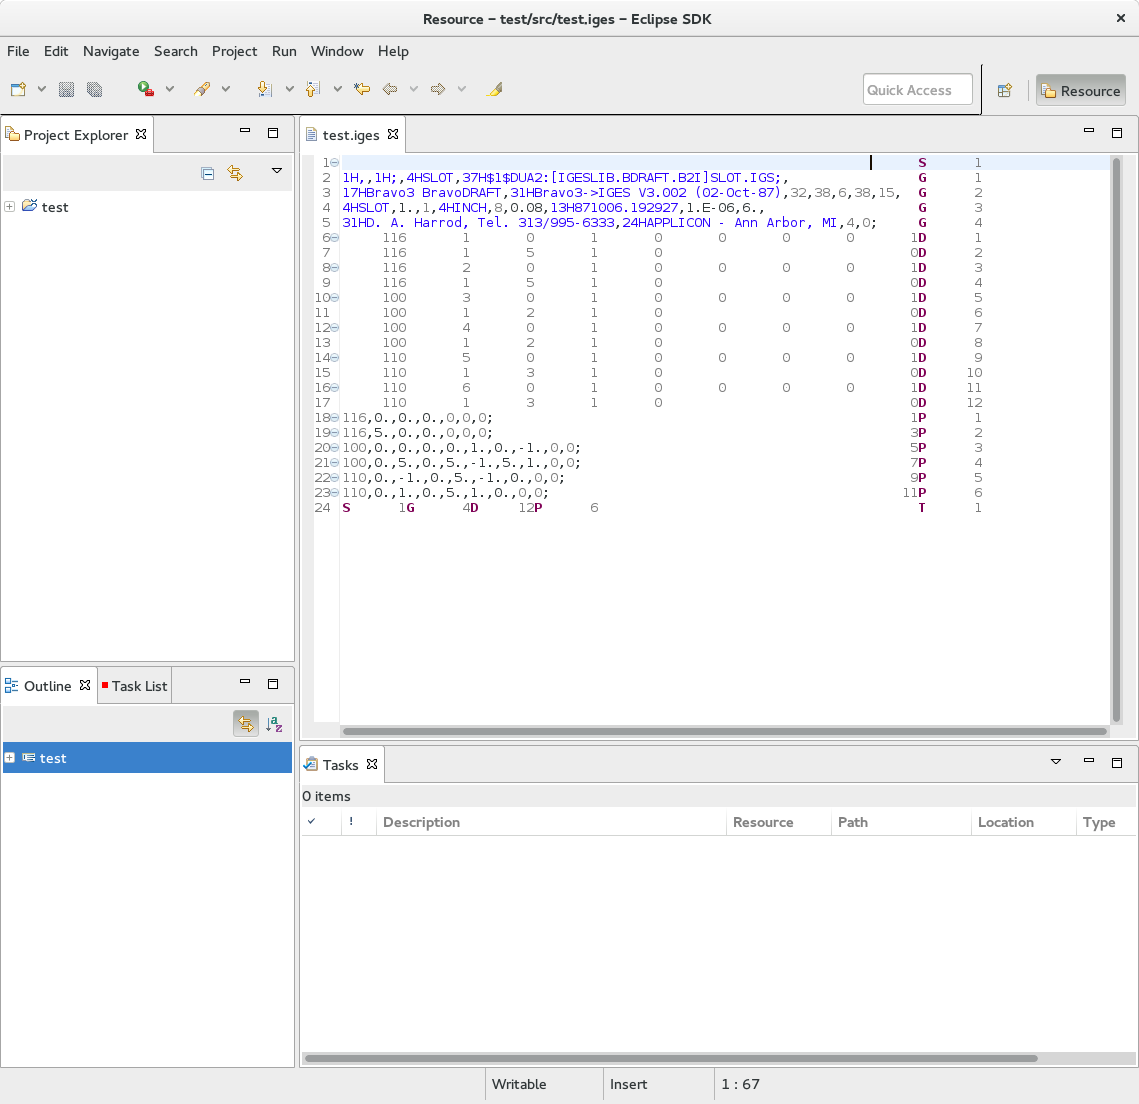
\includegraphics{igesInEditor}

\newpage



